 The general of a circle equation is:
\begin{align}
\norm{\vec{x}-\vec{O}} = r
\end{align}
Substituting the given coordinates
\begin{align}
\norm{\myvec{6\\-6}-\vec{O}}^2 &= r^2 \label{eq:4.2.2_vec_circle_ex} \\
\norm{\myvec{3\\-7}-\vec{O}}^2 &= r^2 \label{eq:4.2.2_vec2_circle_ex}\\
\norm{\myvec{3\\3}-\vec{O}}^2 &= r^2 \label{eq:4.2.2_vec3_circle_ex}
\end{align}

From \eqref{eq:4.2.2_vec_circle_ex}, \eqref{eq:4.2.2_vec2_circle_ex}, \eqref{eq:4.2.2_vec3_circle_ex}:
\begin{align}
\norm{\myvec{3\\-7}-\vec{O}}^2 - \norm{\myvec{6\\-6}-\vec{O}}^2 &= 0 \label{eq:4.2.2_vec4_circle_ex} \\
\norm{\myvec{3\\3}-\vec{O}}^2 - \norm{\myvec{6\\-6}-\vec{O}}^2 &= 0 \label{eq:4.2.2_vec5_circle_ex}
\end{align} 

Simplifying equations \eqref{eq:4.2.2_vec4_circle_ex} and \eqref{eq:4.2.2_vec5_circle_ex}:
\begin{align}
\myvec{3 & 1 \\ 1 & -3 }\vec{O} &= \myvec{7\\9}\\
\myvec{3 & 1 & 7  \\
1 & -3 & 9 
}
&\xleftrightarrow[]{R_1 \leftarrow \frac{R_1}{3}}
\myvec{1 & \frac{1}{3} & \frac{7}{3} \\
1 & -3 & 9 
}\\
&\xleftrightarrow[]{R_2 \leftarrow R_2 - R_1}
\myvec{1 & \frac{1}{3} & \frac{7}{3} \\
1 & -\frac{10}{3} & \frac{20}{3} 
}\\
&\xleftrightarrow[]{R_2 \leftarrow \frac{-3R_2}{10}}
\myvec{1 & \frac{1}{3} & \frac{7}{3} \\
1 & 1 & -2 
}\\
&\xleftrightarrow[]{R_1 \leftarrow R_1-\frac{R_2}{3}}
\myvec{1 & 0 & 3 \\
0 & 1 & -2 
}\\
\therefore \vec{O} = \myvec{3\\-2}
\end{align}

 \begin{figure}[!ht]
\centering
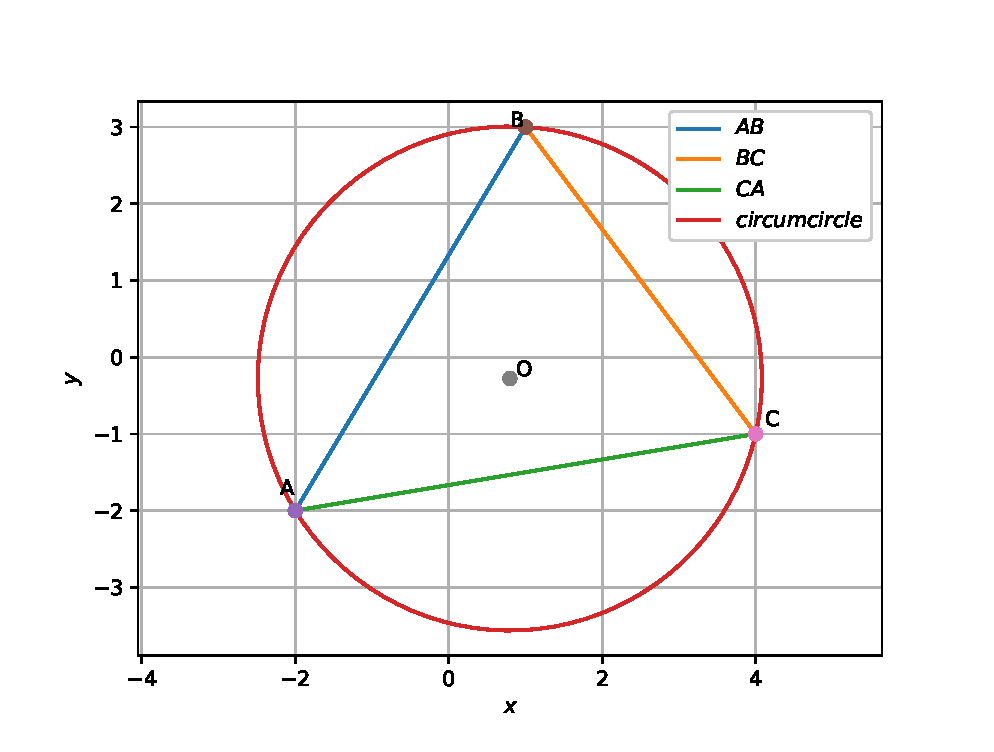
\includegraphics[width=\columnwidth]{./solutions/2/figs/circle_ex/circumcircle.eps}
\caption{}
\label{fig:4.2.2_Circumcircle2_circle_ex}
\end{figure} 

The following Python code generates Fig. \ref{fig:4.2.2_Circumcircle2_circle_ex}

\begin{lstlisting}
solutions/2/codes/circle_ex/circumcircle.py
\end{lstlisting}



